\documentclass{standalone}
\usepackage{pgfplots}
\pgfplotsset{compat=newest}

\begin{document}
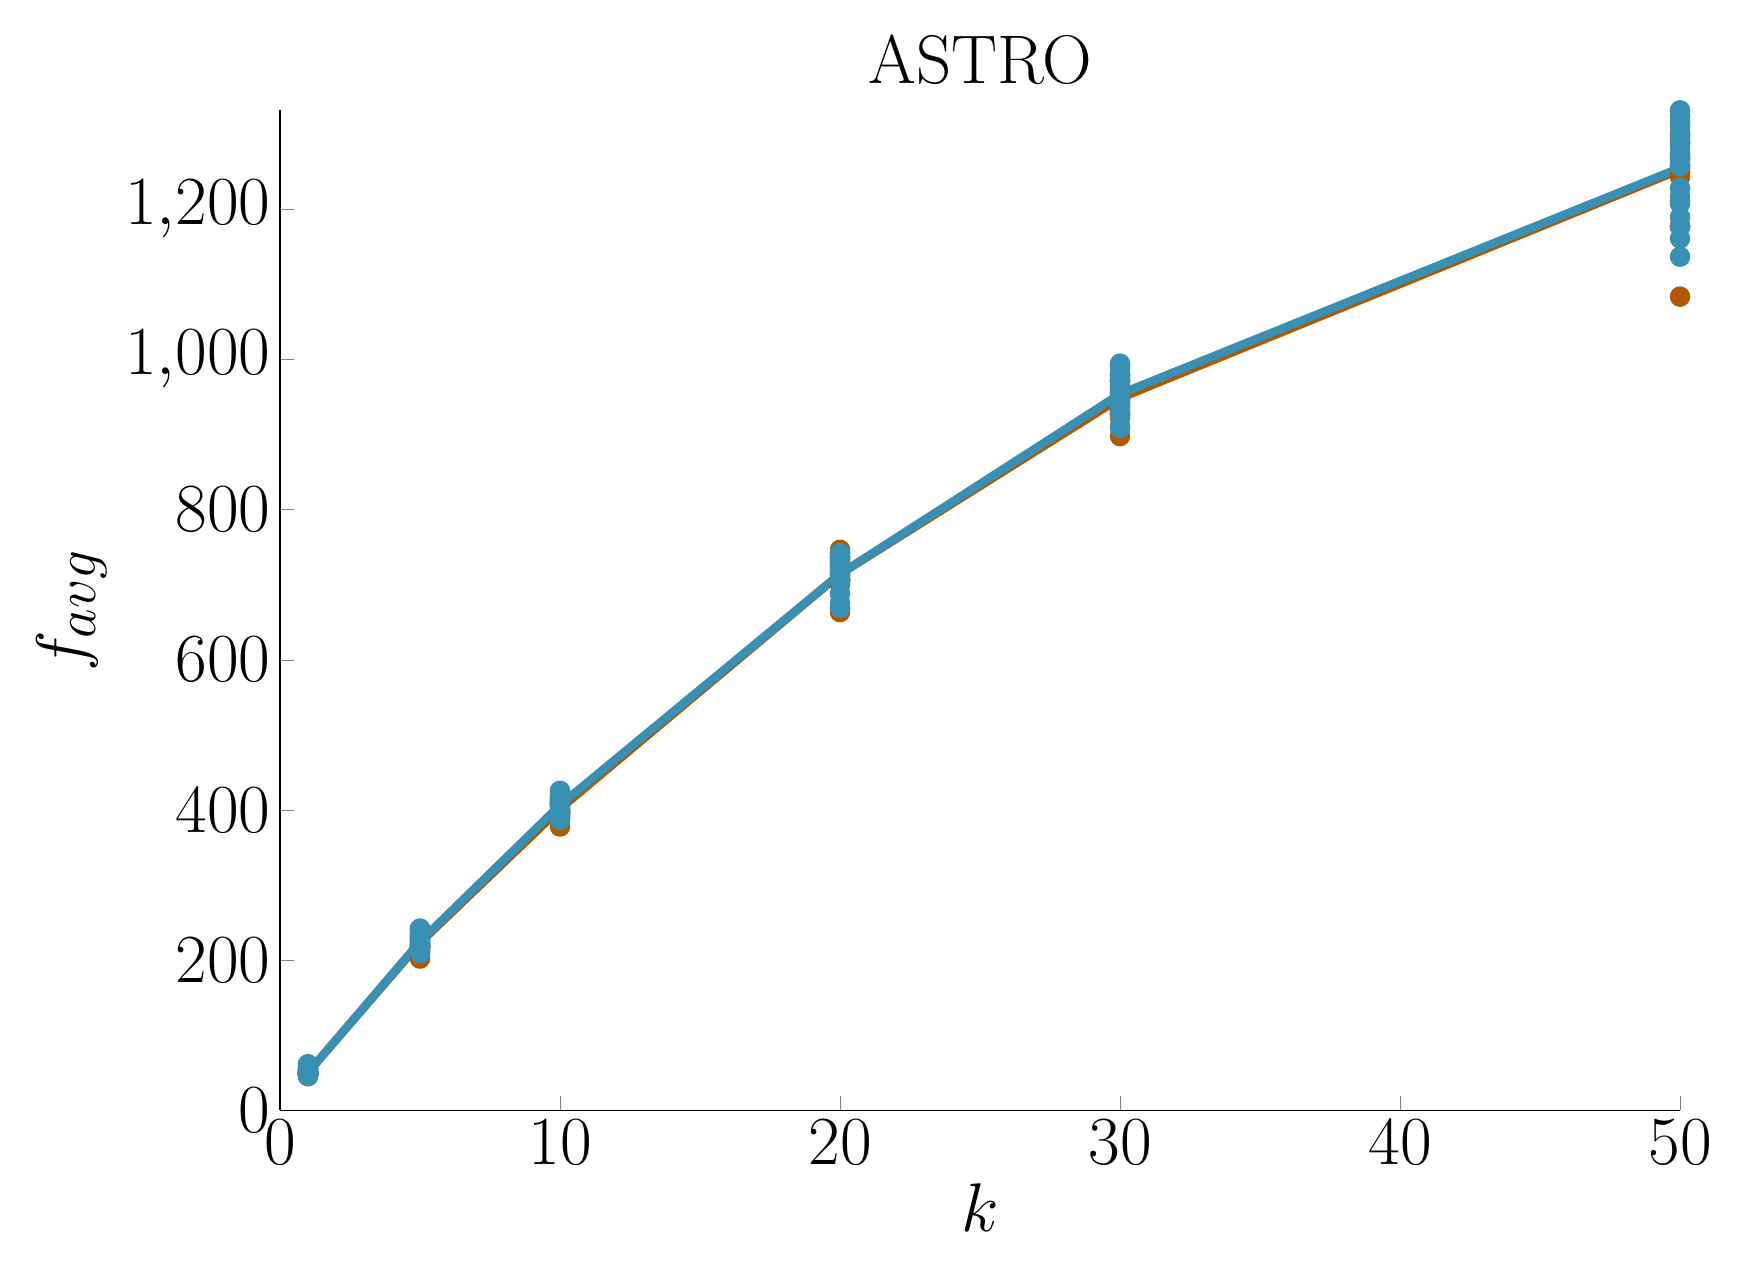
\begin{tikzpicture}

\begin{axis}[%
title style={font=\Huge},
title=ASTRO,
tick label style={font=\Huge},
label style={font=\Huge},
legend style={font=\Huge},
view={0}{90},
max space between ticks=50pt,
width=7in,
height=5in,
scale only axis,
xmin=0, xmax=50,
xtick={0, 10, 20, 30, 40, 50},
xlabel={$k$},
ymin=0, ymax=1331.78,
%ytick={0, 200, 400, 600, 800, 1000},
ylabel={$f_{avg}$},
major tick length=5pt,
axis lines*=left,
legend cell align=left,
clip=false]

\addplot [
only marks,
mark=*,
mark size=3.5pt,
color=orange!70!black,
%solid,
%line width=2pt,
]
coordinates{
(1,45.52)(1,46.02)(1,47.43)(1,47.44)(1,47.7)(1,47.93)(1,48.48)(1,48.52)(1,49.41)(1,49.78)(1,50.06)(1,50.18)(1,50.21)(1,50.64)(1,51.28)(1,52.22)(1,52.83)(1,55.14)(1,56.01)(1,61.17)(5,202.07)(5,209.77)(5,213.32)(5,214.23)(5,217.18)(5,217.23)(5,217.28)(5,218.09)(5,219.39)(5,219.89)(5,220.97)(5,221.98)(5,222.5)(5,229.47)(5,232.66)(5,233.43)(5,236.57)(5,237.72)(5,239.2)(5,241.24)(10,377.93)(10,390.49)(10,390.53)(10,394.02)(10,394.06)(10,395.74)(10,396.27)(10,397.13)(10,397.17)(10,397.26)(10,400.82)(10,403.16)(10,405.35)(10,406.0)(10,407.46)(10,409.64)(10,412.47)(10,416.38)(10,416.45)(10,421.21)(20,663.43)(20,666.98)(20,669.66)(20,700.86)(20,704.42)(20,704.54)(20,706.93)(20,707.01)(20,707.14)(20,712.52)(20,714.5)(20,728.53)(20,728.98)(20,729.09)(20,734.27)(20,735.38)(20,736.42)(20,741.03)(20,742.12)(20,746.6)(30,897.86)(30,910.18)(30,922.83)(30,926.72)(30,927.0)(30,931.41)(30,931.58)(30,937.17)(30,947.25)(30,948.36)(30,952.95)(30,955.54)(30,959.08)(30,962.03)(30,962.39)(30,970.5)(30,973.54)(30,977.69)(30,980.64)(30,992.56)(50,1083.64)(50,1177.16)(50,1177.25)(50,1212.02)(50,1243.34)(50,1248.71)(50,1249.69)(50,1253.98)(50,1255.04)(50,1259.34)(50,1266.66)(50,1268.07)(50,1270.58)(50,1272.3)(50,1287.34)(50,1289.2)(50,1297.97)(50,1299.45)(50,1313.89)(50,1324.91)
};

\addplot [
only marks,
mark=*,
mark size=3.5pt,
color=cyan!70!black,
%solid,
%line width=2pt,
]
coordinates{
(1,45.52)(1,46.02)(1,47.43)(1,47.44)(1,47.7)(1,47.93)(1,48.48)(1,48.52)(1,49.41)(1,49.78)(1,50.06)(1,50.18)(1,50.21)(1,50.64)(1,51.28)(1,52.22)(1,52.83)(1,55.14)(1,56.01)(1,61.17)(5,209.35)(5,211.59)(5,216.7)(5,217.08)(5,217.8)(5,217.96)(5,219.49)(5,219.99)(5,223.23)(5,224.34)(5,225.48)(5,225.95)(5,227.0)(5,228.66)(5,229.7)(5,230.8)(5,232.64)(5,233.72)(5,241.11)(5,242.12)(10,386.61)(10,391.3)(10,396.42)(10,397.84)(10,398.91)(10,399.55)(10,399.87)(10,400.33)(10,405.44)(10,408.14)(10,408.46)(10,409.47)(10,410.43)(10,410.87)(10,411.0)(10,413.66)(10,414.95)(10,416.66)(10,424.78)(10,425.5)(20,669.17)(20,675.47)(20,688.06)(20,705.37)(20,705.99)(20,706.1)(20,711.46)(20,714.83)(20,716.42)(20,716.67)(20,716.7)(20,717.4)(20,721.85)(20,722.49)(20,724.5)(20,726.39)(20,732.61)(20,735.71)(20,737.07)(20,742.55)(30,908.6)(30,910.93)(30,927.14)(30,938.73)(30,939.18)(30,940.93)(30,942.93)(30,946.26)(30,946.57)(30,948.27)(30,951.2)(30,957.39)(30,965.76)(30,970.83)(30,971.17)(30,971.42)(30,979.61)(30,979.65)(30,989.46)(30,994.38)(50,1136.8)(50,1161.09)(50,1176.73)(50,1189.6)(50,1207.55)(50,1217.67)(50,1228.14)(50,1257.36)(50,1257.78)(50,1258.6)(50,1265.13)(50,1274.31)(50,1283.33)(50,1290.52)(50,1302.62)(50,1309.09)(50,1312.06)(50,1318.37)(50,1323.93)(50,1331.78)
};

\addplot [
color=orange!70!black,
solid,
line width=3pt
]
coordinates{
(1,50.3985)(5,223.2095)(10,401.477)(20,714.0205)(30,948.364)(50,1252.527)
};

\addplot [
color=cyan!70!black,
solid,
line width=3pt
]
coordinates{
(1,50.3985)(5,224.7355)(10,406.5095)(20,714.3405)(30,954.0205)(50,1255.123)
};


\end{axis}
\end{tikzpicture}
\end{document}
